\chapter{Introduction}
\lecture{1}{9/07--9/10}{}

\section{Equations Containing No Derivatives, and Differential Equations}

\source{Lecture material; cf.\ Boyce §1.1}

Before saying what a differential equation \emph{is}, it pays to say what it is
\emph{not}.

\begin{definition}[Equation containing no derivatives]
	An \vocab{algebraic equation} (more generally, an equation containing no
	derivatives) is a relation among numbers, such as
	\[
		x^2 - 5x + 6 = 0
		\qquad\text{or}\qquad
		\begin{cases}
			2x + 3y = 7, \\
			x - y = 1.
		\end{cases}
	\]
	To \emph{solve} it is to find the numbers --- here \(x \in \{2,3\}\), and
	\((x,y) = (2,1)\) --- that make it true.
\end{definition}

\begin{definition}[Differential equation]
	A \vocab{differential equation} is an equation relating an unknown
	\emph{function} to one or more of its derivatives, such as
	\[
		\frac{\dd y}{\dd t} = y.
	\]
	To \emph{solve} it is to find the \emph{functions} --- here
	\(y(t) = ce^{t}\) for any constant \(c\) --- that make it true on some interval.
\end{definition}

\begin{moral}
	An algebraic equation asks \emph{which number?} A differential equation asks
	\emph{which function?} The unknown has been promoted from a point to a whole curve.
\end{moral}

\begin{observation}
	This promotion changes the shape of the answer. The solution set of a polynomial
	equation is a finite list of numbers; the solution set of a differential equation is
	typically an infinite \emph{family} of functions, indexed by one or more arbitrary
	constants. The reason is that solving a differential equation involves integrating,
	and every integration brings with it a constant of integration.
\end{observation}

\begin{eg}
	Compare:
	\begin{center}
		\begin{tabular}{@{}lll@{}}
			\toprule
			                 & \(x^2 - 5x + 6 = 0\) & \(y' = y\)                       \\
			\midrule
			unknown          & a number \(x\)       & a function \(y(\cdot)\)          \\
			solution set     & \(\{2, 3\}\)         & \(\{\,ce^{t} : c \in \mathbb{R}\,\}\) \\
			how to pin it down & --- (already finite) & one extra condition, e.g.\ \(y(0)=1\) \\
			\bottomrule
		\end{tabular}
	\end{center}
\end{eg}

\begin{definition}[Initial condition, initial value problem]
	A condition of the form \(y(t_0) = y_0\) is an \vocab{initial condition}. A
	differential equation together with an initial condition is an \vocab{initial value
		problem} (IVP). Geometrically, the initial condition selects the one curve of the
	family that passes through the point \((t_0, y_0)\).
\end{definition}

\begin{note}[Historical background I: Newton, Leibniz, the Bernoullis]
	The subject originated with the calculus of \textsc{Isaac Newton} (1643--1727) and
	\textsc{Gottfried Wilhelm Leibniz} (1646--1716). Newton identified three forms of
	first-order equation, \(\dd y/\dd x = f(x)\), \(\dd y/\dd x = f(y)\) and
	\(\dd y/\dd x = f(x,y)\), solving the last by infinite series when \(f\) is a
	polynomial. Leibniz gave us the notation \(\dd y/\dd x\) and the integral sign, and
	discovered separation of variables (1691) and the solution of first-order linear
	equations (1694). The brothers \textsc{Jakob} (1654--1705) and \textsc{Johann
		Bernoulli} (1667--1748) of Basel developed the methods further; the brachistochrone
	problem, solved by both (and by Leibniz, Newton and l'Hôpital), was a famous source of
	friction between them.
\end{note}

\section{Static Viewpoint and Dynamic Viewpoint}

\source{Lecture material; not in Boyce}

The whole subject rests on one change of perspective.

\begin{moral}
	\textbf{Static viewpoint:} describe a quantity by its \emph{value}.\\
	\textbf{Dynamic viewpoint:} describe a quantity by its \emph{rate of change}, together
	with where it started.
\end{moral}

The second description is usually the one we can actually obtain, and --- by the
fundamental theorem of calculus --- it contains exactly as much information as the first.
Five illustrations.

\subsection{Five Illustrations}

\subsubsection*{1. Salary}

Two offers: company \(A\) starts you at \(60\)k with a raise of \(2\)k per year;
company \(B\) starts you at \(40\)k with a raise of \(5\)k per year. Statically \(A\) is
better. Dynamically \(B\) is better, and after
\[
	60 + 2t = 40 + 5t \iff t = \frac{20}{3} \approx 6.7 \text{ years}
\]
\(B\) overtakes \(A\) and never looks back.

\begin{figure}[H]
	\centering
	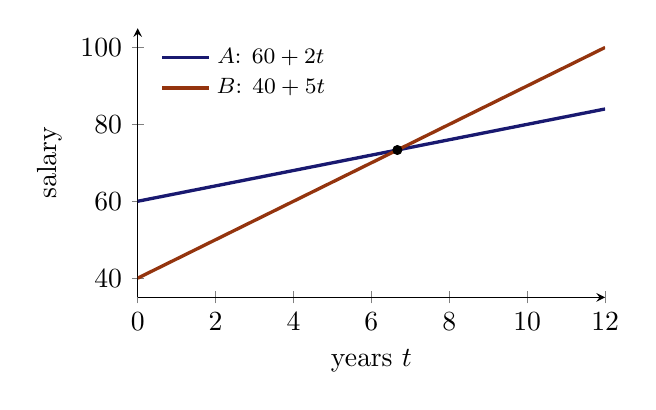
\begin{tikzpicture}
		\begin{axis}[
				width=0.62\textwidth, height=5cm,
				xlabel={years $t$}, ylabel={salary},
				xmin=0, xmax=12, ymin=35, ymax=105,
				axis lines=left, legend pos=north west,
				legend style={draw=none, font=\footnotesize, fill=none},
			]
			\addplot[very thick, MidnightBlue, domain=0:12, samples=2]{60+2*x};
			\addlegendentry{$A$: $60 + 2t$}
			\addplot[very thick, RawSienna, domain=0:12, samples=2]{40+5*x};
			\addlegendentry{$B$: $40 + 5t$}
			\addplot[only marks, mark=*, mark size=1.6pt, black]
			coordinates {(6.667,73.33)};
		\end{axis}
	\end{tikzpicture}
	\caption{The static comparison (values at \(t=0\)) and the dynamic comparison
		(slopes) give opposite answers.}
\end{figure}

\begin{moral}
	Over any horizon long enough to matter, the \emph{derivative} beats the
	\emph{value}.
\end{moral}

\subsubsection*{2. Friends and careers}

A popular slogan says that you become the average of the people you spend your time
with. Take it literally: let \(x(t)\) measure some trait of yours and let \(m\) be the
average of that trait over the people around you. The slogan is not the statement
\(x = m\) (that is false at every instant); it is the statement that you \emph{drift
	towards} \(m\) at a rate proportional to how far away you are:
\begin{equation}\label{eq:friends}
	\frac{\dd x}{\dd t} = k\,(m - x), \qquad k > 0.
\end{equation}

\begin{observation}
	Equation~\eqref{eq:friends} is literally Newton's law of cooling
	(\autoref{sec:relax}), with your environment playing the role of the ambient
	temperature. Its solution is
	\(x(t) = m + (x_0 - m) e^{-kt}\): the starting value \(x_0\) is forgotten
	exponentially fast, and the only thing that survives in the long run is \(m\). So a
	dynamic model says something a static one cannot --- \emph{who you are around
		eventually matters more than where you started}, and the rate \(k\) decides how fast
	``eventually'' arrives.
\end{observation}

\subsubsection*{3. The fundamental theorem of calculus}

The dictionary translating between the two viewpoints is the fundamental theorem of
calculus:
\[
	F(b) - F(a) = \int_{a}^{b} F'(t) \dd t.
\]

\begin{intuition}
	Read from right to left, this says: \emph{knowing the rate everywhere, plus one
		value, recovers the function everywhere}. In other words, the fundamental theorem of
	calculus is exactly the solution of the simplest possible initial value problem,
	\[
		\frac{\dd y}{\dd t} = f(t), \quad y(t_0) = y_0
		\qquad\Longrightarrow\qquad
		y(t) = y_0 + \int_{t_0}^{t} f(s) \dd s.
	\]
	Everything in this course is an attempt to do the same thing when the right-hand side
	is allowed to depend on \(y\) as well as on \(t\).
\end{intuition}

\subsubsection*{4. Inequality proofs via derivatives}

To prove \(f(x) \geq g(x)\) for all \(x \geq a\), it suffices to check the inequality
\emph{once}, at \(x = a\), and then compare \emph{rates}.

\begin{proposition}\label{prop:ineq}
	Let \(f, g\) be differentiable on \([a, \infty)\). If \(f(a) \geq g(a)\) and
	\(f'(x) \geq g'(x)\) for all \(x > a\), then \(f(x) \geq g(x)\) for all \(x \geq a\).
\end{proposition}

\begin{proof}
	Let \(h = f - g\). Then \(h(a) \geq 0\) and \(h' \geq 0\) on \((a,\infty)\), so \(h\)
	is nondecreasing; hence \(h(x) \geq h(a) \geq 0\) for \(x \geq a\).
\end{proof}

\begin{eg}
	To prove \(e^{x} \geq 1 + x\) for \(x \geq 0\): at \(x = 0\) both sides equal \(1\),
	and \(\frac{\dd}{\dd x} e^{x} = e^{x} \geq 1 = \frac{\dd}{\dd x}(1+x)\) for
	\(x \geq 0\). Done. Similarly \(\sin x \leq x\) and \(\ln(1+x) \leq x\) for
	\(x \geq 0\).
\end{eg}

\begin{remark}
	\autoref{prop:ineq} is the baby case of a \vocab{comparison theorem}: one controls a
	solution of a differential \emph{inequality} by a solution of a differential
	\emph{equation}. The same idea, run at full strength, is how one proves that
	solutions of nonlinear equations stay bounded.
\end{remark}

\subsubsection*{5. Nature loves to use derivatives}

Almost every law of nature is stated as a rate, not as a value:
\begin{center}
	\begin{tabular}{@{}ll@{}}
		\toprule
		Newton's second law     & \(m \ddot{\vb{x}} = \vb{F}\)                       \\
		Radioactive decay       & \(\dot{N} = -\lambda N\)                           \\
		Newton's law of cooling & \(\dot{u} = -k(u - T)\)                            \\
		Fourier's law of heat   & \(\vb{q} = -\kappa \grad u\)                       \\
		Fick's law of diffusion & \(\vb{J} = -D \grad c\)                            \\
		\bottomrule
	\end{tabular}
\end{center}

\begin{intuition}
	Why should this be? Because nature is \emph{local}. A particle does not know where it
	will be in an hour, or where it was yesterday; it only knows the forces acting on it
	right now. A law of nature can therefore only be a statement about the present
	instant --- and a statement about how a quantity is changing at the present instant is
	precisely a statement about its derivative.
\end{intuition}

\begin{eg}[A falling object]\label{eg:fall}
	An object of mass \(m\) falls in the atmosphere near sea level. Formulate a
	differential equation describing its motion.
\end{eg}

\begin{proof}[Model]
	Let \(t\) denote time (seconds) and let \(v = v(t)\) be the velocity
	(\si{\metre\per\second}), taken \emph{positive downwards}. Thus \(t\) is the
	independent variable and \(v\) is the dependent variable.

	Newton's second law states that
	\[
		F = ma = m\frac{\dd v}{\dd t},
	\]
	where \(F\) is the net force on the object. Two forces act:
	\begin{itemize}
		\item gravity, of magnitude \(mg\), acting downwards (positive), where
		      \(g \approx \SI{9.8}{\metre\per\second\squared}\);
		\item drag (air resistance), which we \emph{assume} to be proportional to the
		      velocity, of magnitude \(\gamma v\), acting upwards (negative). The constant
		      \(\gamma > 0\) is the \vocab{drag coefficient}, with units of
		      \(\si{\kilogram\per\second}\).
	\end{itemize}
	Hence \(F = mg - \gamma v\), and the model is
	\begin{equation}\label{eq:fall}
		m \frac{\dd v}{\dd t} = mg - \gamma v.
	\end{equation}
\end{proof}

\begin{note}
	Equation~\eqref{eq:fall} contains three constants \(m\), \(g\), \(\gamma\). We call
	\(m\) and \(\gamma\) \vocab{parameters}: they depend on the particular falling object
	and may range over many values during an experiment. By contrast \(g\) is a
	\vocab{physical constant}, the same for every object.
\end{note}

Taking \(m = \SI{10}{\kilogram}\) and \(\gamma = \SI{2}{\kilogram\per\second}\),
equation~\eqref{eq:fall} becomes
\begin{equation}\label{eq:fall-num}
	\frac{\dd v}{\dd t} = 9.8 - \frac{v}{5}.
\end{equation}

\subsection{Direction Fields: Seeing the Dynamics Without Solving}

\source{Boyce §1.1}

We do not yet know how to solve~\eqref{eq:fall-num}. The dynamic viewpoint says we
should not need to: the equation already tells us the slope of the solution at every
point of the plane.

\begin{definition}[Direction field]
	Consider a first-order equation in the form
	\begin{equation}\label{eq:general-first-order}
		\frac{\dd y}{\dd t} = f(t, y),
	\end{equation}
	where \(f\) --- sometimes called the \vocab{rate function} --- is a given function of
	the two variables \(t\) and \(y\). The \vocab{direction field} (or \vocab{slope
		field}) of~\eqref{eq:general-first-order} is obtained by drawing, at each point
	\((t, y)\) of a rectangular grid, a short line segment of slope \(f(t, y)\).
\end{definition}

\begin{intuition}
	A solution of~\eqref{eq:general-first-order} is a function \(y = y(t)\) whose graph
	is a curve in the \(ty\)-plane. At each of its points, that curve has slope
	\(f(t,y)\). Hence \textbf{every line segment of the direction field is tangent to
		the solution curve through that point}: the direction field shows the ``flow'' that
	the solution curves must follow.
\end{intuition}

\begin{remark}
	Two practical points deserve emphasis.
	\begin{enumerate}[(i)]
		\item Constructing a direction field requires \emph{no} solution
		      of~\eqref{eq:general-first-order}; one only evaluates \(f(t,y)\) many times.
		      So direction fields can be drawn even for equations that are very hard --- or
		      impossible --- to solve in closed form.
		\item Repeated evaluation and plotting is exactly the kind of task a computer does
		      well; a grid of a few hundred points usually suffices.
	\end{enumerate}
\end{remark}

\begin{eg}[Behaviour of solutions of~\eqref{eq:fall-num}]
	Read off from~\eqref{eq:fall-num}: if \(v = 40\) then \(\dd v/\dd t = 1.8 > 0\); if
	\(v = 50\) then \(\dd v/\dd t = -0.2 < 0\); if \(v = 60\) then \(\dd v/\dd t = -2.2 <
	0\). So there is a critical value of \(v\) separating solutions that increase from
	those that decrease, found by setting \(\dd v/\dd t = 0\):
	\[
		9.8 - \frac{v}{5} = 0 \iff v = 5 \cdot 9.8 = \SI{49}{\metre\per\second}.
	\]
\end{eg}

\begin{definition}[Equilibrium solution]
	A constant solution \(y(t) \equiv c\) of \(\dd y/\dd t = f(t,y)\) is called an
	\vocab{equilibrium solution}. Equivalently, \(c\) is a root of \(f(t, c) = 0\)
	for all \(t\).
\end{definition}

For~\eqref{eq:fall-num} the equilibrium solution is \(v(t) \equiv 49\): substituting it
makes both sides zero. Physically it is the perfect balance between gravity and drag, and
since all other solutions appear to converge to it, it is called the \vocab{terminal
	velocity}.

\begin{figure}[H]
	\centering
	\begin{tikzpicture}
		\begin{axis}[
				width=0.62\textwidth, height=6.2cm,
				xlabel={$t$}, ylabel={$v$},
				xmin=0, xmax=10, ymin=39, ymax=61,
				ytick={40,45,50,55,60},
				axis lines=left,
			]
			\foreach \X in {0.5,1.5,...,9.5}{
					\foreach \Y in {40,42,...,60}{
							\pgfmathsetmacro{\Sl}{9.8-\Y/5}%
							\slopemark{RawSienna!80}{\X}{\Y}{\Sl}{0.992}{0.2818}
						}
				}
			\addplot[very thick, blue, domain=0:10, samples=2]{49};
			\node[blue, anchor=south west, font=\footnotesize] at (axis cs:7.5,49.3) {$v=49$};
		\end{axis}
	\end{tikzpicture}
	\caption{Direction field and equilibrium solution of
		\(\dd v/\dd t = 9.8 - v/5\). The equilibrium \(v = 49\) \emph{attracts} the
		other solutions.}
	\label{fig:dirfield-fall}
\end{figure}

\section{Examples}

\source{Boyce §1.1 (population, linear model); the remaining models are lecture material}

\subsection{Population Growth}

\begin{eg}[Field mice and owls]
	A population of field mice inhabits a rural area. In the absence of predators we
	assume the population grows at a rate proportional to the current population: if
	\(p(t)\) denotes the population at time \(t\), then
	\begin{equation}\label{eq:mice-basic}
		\frac{\dd p}{\dd t} = r p,
	\end{equation}
	where the proportionality factor \(r\) is the \vocab{rate constant} or \vocab{growth
		rate}. Suppose \(t\) is measured in months and \(r = 0.5/\text{month}\).

	Now suppose owls in the neighbourhood kill \(15\) field mice per \emph{day}. Since
	time is measured in months, the predation term is \(-450\) per month, and the model
	becomes
	\begin{equation}\label{eq:mice}
		\frac{\dd p}{\dd t} = \frac{p}{2} - 450.
	\end{equation}
\end{eg}

Setting \(\dd p/\dd t = 0\) gives the equilibrium solution \(p(t) \equiv 900\), at which
growth and predation exactly balance.

\begin{figure}[H]
	\centering
	\begin{tikzpicture}
		\begin{axis}[
				width=0.62\textwidth, height=6.2cm,
				xlabel={$t$}, ylabel={$p$},
				xmin=0, xmax=5, ymin=795, ymax=1005,
				ytick={800,850,900,950,1000},
				axis lines=left,
			]
			\foreach \X in {0.25,0.75,...,4.75}{
					\foreach \Y in {800,820,...,1000}{
							\pgfmathsetmacro{\Sl}{\Y/2-450}%
							\slopemark{RawSienna!80}{\X}{\Y}{\Sl}{1.984}{0.02952}
						}
				}
			\addplot[very thick, blue, domain=0:5, samples=2]{900};
			\node[blue, anchor=south west, font=\footnotesize] at (axis cs:3.6,903) {$p=900$};
		\end{axis}
	\end{tikzpicture}
	\caption{Direction field and equilibrium solution of
		\(\dd p/\dd t = p/2 - 450\). Here the equilibrium \(p = 900\) \emph{repels} the
		other solutions.}
	\label{fig:dirfield-mice}
\end{figure}

\begin{moral}
	In both examples so far the equilibrium solution separates increasing solutions from
	decreasing ones. But the two behave oppositely: solutions of~\eqref{eq:fall-num} are
	\emph{attracted} by the equilibrium, while solutions of~\eqref{eq:mice} are
	\emph{repelled} by it. In the latter case the equilibrium itself will never be
	observed in practice --- yet it is still the key to understanding the picture.
\end{moral}

\begin{remark}[Limitations]
	Model~\eqref{eq:fall-num} is valid only while the object falls freely; at large
	velocities the assumption that drag is \emph{linear} in \(v\) must be replaced by a
	nonlinear one. Model~\eqref{eq:mice} eventually predicts either a negative number of
	mice (if \(p < 900\)) or an absurdly large one (if \(p > 900\)), so it becomes
	unacceptable after a fairly short time. A better population model --- the
	\vocab{logistic equation} --- appears in Boyce §2.5.
\end{remark}

\subsection{Relaxation Processes and Equilibria}\label{sec:relax}

All the models below are the same equation wearing different clothes. We solve it once.

\subsubsection*{The linear model}

\begin{theorem}[General solution of \(y' = ay - b\)]\label{thm:linear-const}
	Let \(a \neq 0\). The differential equation
	\begin{equation}\label{eq:linear-const}
		\frac{\dd y}{\dd t} = ay - b
	\end{equation}
	has general solution
	\begin{equation}\label{eq:gensol}
		y(t) = \frac{b}{a} + c e^{at}, \qquad c \in \mathbb{R} \text{ arbitrary},
	\end{equation}
	and the solution of the initial value problem \(y' = ay-b\), \(y(0) = y_0\) is
	\begin{equation}\label{eq:ivpsol}
		y(t) = \frac{b}{a} + \left( y_0 - \frac{b}{a} \right) e^{at}.
	\end{equation}
\end{theorem}

The computation you would actually perform is to divide by \(y - b/a\) and integrate a
logarithm. That works, but it needs an argument to justify it (\autoref{rmk:logcare}
below), so we first give a proof that avoids division altogether.

\begin{proof}
	\textbf{Step 1: every solution has the form~\eqref{eq:gensol}.}
	Let \(y\) be \emph{any} solution of~\eqref{eq:linear-const} on an interval \(I\), and
	define the auxiliary function
	\begin{equation}\label{eq:auxw}
		w(t) \coloneq \left( y(t) - \frac{b}{a} \right) e^{-at},
		\qquad t \in I.
	\end{equation}
	Differentiating with the product rule, and then using \(y' = ay - b\),
	\[
		w'(t)
		= y'(t) e^{-at} - a\left( y(t) - \frac{b}{a} \right) e^{-at}
		= e^{-at}\Bigl[\, \underbrace{y'(t)}_{=\,ay(t)-b} - \,a y(t) + b \,\Bigr]
		= e^{-at} \cdot 0 = 0
	\]
	for every \(t \in I\). A function with vanishing derivative on an \emph{interval} is
	constant, so \(w(t) = c\) for some \(c \in \mathbb{R}\) and all \(t \in I\). Solving
	\eqref{eq:auxw} for \(y\) gives exactly~\eqref{eq:gensol}.

	\textbf{Step 2: every function of the form~\eqref{eq:gensol} is a solution.}
	If \(y(t) = \frac ba + ce^{at}\), then \(y'(t) = ac\,e^{at}\), while
	\[
		ay(t) - b = a\!\left( \frac{b}{a} + c e^{at} \right) - b
		= \cancel{b} + ac\,e^{at} - \cancel{b} = ac\,e^{at} = y'(t). \checkmark
	\]

	\textbf{Step 3: the initial condition.} Setting \(t = 0\) in~\eqref{eq:gensol} gives
	\(y_0 = \frac ba + c\), i.e.\ \(c = y_0 - \frac ba\), which is~\eqref{eq:ivpsol}.
\end{proof}

\begin{remark}
	Step 1 never divides by anything and never takes a logarithm, so no value of \(y\) has
	to be excluded: the equilibrium solution \(y \equiv b/a\) simply appears as the case
	\(c = 0\), with no special pleading. The function \(e^{-at}\)
	in~\eqref{eq:auxw} is not magic --- it is the \vocab{integrating factor} of
	\autoref{thm:integrating-factor}, met here for the first time.
\end{remark}

\begin{remark}[What the logarithm computation really proves]\label{rmk:logcare}
	Here is the usual computation. Assuming \(y(t) \neq b/a\), rewrite
	\eqref{eq:linear-const} as
	\[
		\frac{\dd y/\dd t}{\,y - \frac{b}{a}\,} = a,
	\]
	recognise the left-hand side as
	\(\dfrac{\dd}{\dd t} \ln\abs{y - \frac{b}{a}}\) by the chain rule, and integrate:
	\begin{equation}\label{eq:logstep}
		\ln\abs{y(t) - \frac{b}{a}} = at + C
		\implies
		\abs{y(t) - \frac{b}{a}} = e^{C} e^{at}
		\implies
		y(t) - \frac{b}{a} = \pm e^{C} e^{at}.
	\end{equation}
	It gets the right answer, but as it stands it has \emph{two} gaps.
	\begin{enumerate}[(i)]
		\item It divides by \(y - b/a\), so it says nothing about a solution that takes the
		      value \(b/a\) somewhere. The equilibrium solution has to be put back by hand,
		      and since \(e^{C} > 0\) the last step of~\eqref{eq:logstep} never produces
		      \(c = 0\) on its own.
		\item \textbf{The sign in~\eqref{eq:logstep} is chosen \emph{locally}.} Removing an
		      absolute value is legitimate only on an interval where \(y - b/a\) keeps a
		      fixed sign. If \(y\) were above \(b/a\) for some times and below it for others,
		      \eqref{eq:logstep} would give \(c = +e^{C}\) on some subintervals and
		      \(c = -e^{C}\) on others --- and there would be no single constant \(c\), so
		      \eqref{eq:gensol} would be false.
	\end{enumerate}
	Gap (ii) is the serious one, and it is exactly the right thing to worry about. It
	closes because the bad case cannot occur:
\end{remark}

\begin{corollary}[A solution never crosses the equilibrium]\label{cor:nocross}
	Let \(y\) be a solution of~\eqref{eq:linear-const} on an interval \(I\). Then
	\emph{exactly one} of the following holds:
	\[
		\text{(a) } y(t) = \frac{b}{a} \ \ \forall t \in I,
		\qquad
		\text{(b) } y(t) > \frac{b}{a} \ \ \forall t \in I,
		\qquad
		\text{(c) } y(t) < \frac{b}{a} \ \ \forall t \in I.
	\]
	In particular \(y - b/a\) has a constant sign, so the sign chosen
	in~\eqref{eq:logstep} is the \emph{same} for all \(t \in I\), and the logarithm
	computation is valid after all.
\end{corollary}

\begin{proof}
	By Step 1 of the proof above, \(y(t) - \frac ba = c\,e^{at}\) for a single constant
	\(c\). Since \(e^{at} > 0\) for every \(t\), the sign of \(y(t) - \frac ba\) equals
	the sign of \(c\) at every \(t\): the three cases are \(c = 0\), \(c > 0\), \(c < 0\).
\end{proof}

\begin{intuition}
	Geometrically: the horizontal line \(y = b/a\) is itself an integral curve, and
	\autoref{cor:nocross} says no other integral curve ever touches it. It acts as a
	\emph{barrier} dividing the plane into two halves, and a solution is trapped in
	whichever half it starts in. Look again at the direction fields on
	pages~\pageref{fig:dirfield-fall} and~\pageref{fig:dirfield-mice}: above the
	equilibrium every segment points one way and below it every segment points the other,
	and nothing ever gets across.

	This is a first instance of something general. Through each point of the plane there
	passes exactly \emph{one} solution curve (Boyce §2.4), so two distinct solutions can
	never meet. A solution meeting the constant solution \(y \equiv b/a\) at one instant
	would have to \emph{be} it --- which is case (a).
\end{intuition}

\begin{eg}[Concretely]
	For the field mice, \(\dd p/\dd t = \frac p2 - 450\) has equilibrium \(p = 900\) and
	general solution \(p(t) = 900 + ce^{t/2}\). A population starting at \(p_0 = 850\)
	has \(c = -50 < 0\), so \(p(t) = 900 - 50e^{t/2}\) stays strictly below \(900\)
	forever --- it does not approach \(900\) from below and then overshoot; it runs away
	downwards. A population starting at \(p_0 = 950\) has \(c = +50\) and stays strictly
	above. No solution is ever on both sides.
\end{eg}

\begin{definition}[General solution, integral curves]
	For \(a \neq 0\), expression~\eqref{eq:gensol} contains \emph{all} solutions
	of~\eqref{eq:linear-const} and is called the \vocab{general solution}. Its geometric
	representation is an infinite family of curves called \vocab{integral curves}, one
	for each value of \(c\). Satisfying an initial condition amounts to selecting the
	integral curve through the given initial point.
\end{definition}

\begin{exercise}
	Find the general solution of~\eqref{eq:linear-const} in the remaining case \(a = 0\).
	(Formula~\eqref{eq:gensol} does not apply.)
\end{exercise}

It is worth rewriting~\eqref{eq:ivpsol} in the form that makes the dynamics obvious. Put
\(y_{\mathrm{eq}} = b/a\) and \(k = -a\):

\begin{corollary}[Relaxation form]\label{cor:relax}
	The initial value problem
	\begin{equation}\label{eq:relax}
		\frac{\dd y}{\dd t} = -k\left( y - y_{\mathrm{eq}} \right), \qquad y(0) = y_0
	\end{equation}
	has the unique solution
	\begin{equation}\label{eq:relax-sol}
		y(t) = y_{\mathrm{eq}} + \left( y_0 - y_{\mathrm{eq}} \right) e^{-kt}.
	\end{equation}
	If \(k > 0\), then \(y(t) \to y_{\mathrm{eq}}\) as \(t \to \infty\): the equilibrium
	is \vocab{stable} (attracting). If \(k < 0\) it is \vocab{unstable} (repelling).
\end{corollary}

\begin{definition}[Relaxation time]
	For \(k > 0\), the quantity \(\tau = 1/k\) is the \vocab{relaxation time} (or
	\vocab{time constant}) of~\eqref{eq:relax}: it is the time in which the deviation
	\(y - y_{\mathrm{eq}}\) shrinks by a factor of \(e\). After \(3\tau\) about \(95\%\)
	of the initial deviation is gone, and after \(5\tau\) about \(99\%\).
\end{definition}

\begin{figure}[H]
	\centering
	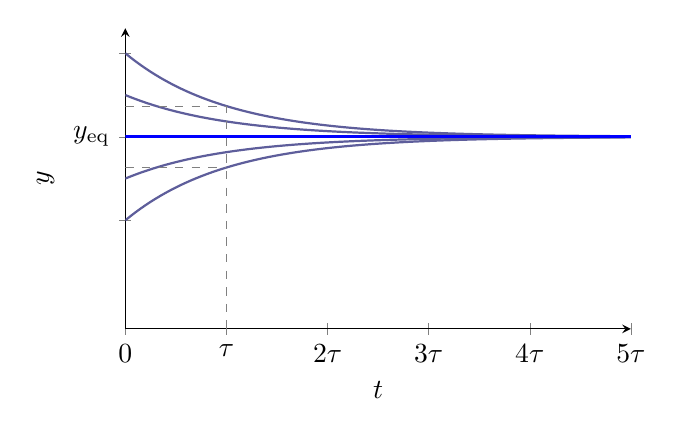
\begin{tikzpicture}
		\begin{axis}[
				width=0.66\textwidth, height=5.4cm,
				xlabel={$t$}, ylabel={$y$},
				xmin=0, xmax=5, ymin=-1.3, ymax=2.3,
				ytick={0,1,2}, yticklabels={,$y_{\mathrm{eq}}$,},
				xtick={0,1,2,3,4,5},
				xticklabels={$0$,$\tau$,$2\tau$,$3\tau$,$4\tau$,$5\tau$},
				axis lines=left,
			]
			\foreach \Z in {-1,-0.5,0.5,1}{
					\addplot[thick, MidnightBlue!70, domain=0:5, samples=100]
					{1+\Z*exp(-x)};
				}
			\addplot[very thick, blue, domain=0:5, samples=2]{1};
			\draw[gray, dashed] (axis cs:0,1.3679) -- (axis cs:1,1.3679)
			-- (axis cs:1,-1.3);
			\draw[gray, dashed] (axis cs:0,0.6321) -- (axis cs:1,0.6321);
		\end{axis}
	\end{tikzpicture}
	\caption{Relaxation towards a stable equilibrium: every solution
		of~\eqref{eq:relax} forgets its initial value exponentially, on the time scale
		\(\tau = 1/k\).}
\end{figure}

\begin{eg}[The falling object, solved]
	Equation~\eqref{eq:fall} is~\eqref{eq:linear-const} with \(a = -\gamma/m\) and
	\(b = -g\), so by~\eqref{eq:ivpsol}
	\[
		v(t) = \frac{mg}{\gamma} + \left( v_0 - \frac{mg}{\gamma} \right)
		e^{-\gamma t/m}.
	\]
	The terminal velocity is \(v_{\mathrm{eq}} = mg/\gamma\) and the relaxation time is
	\(\tau = m/\gamma\): for a given mass, more drag means faster convergence.
\end{eg}

\begin{eg}[The falling object, quantitatively]
	Let \(m = \SI{10}{\kilogram}\), \(\gamma = \SI{2}{\kilogram\per\second}\), so that
	\(\dd v/\dd t = 9.8 - v/5\), and drop the object (\(v(0) = 0\)) from a height of
	\SI{300}{\metre}. How long does it take to reach the ground, and how fast is it then
	moving?
\end{eg}

\begin{proof}[Solution]
	Here \(v_{\mathrm{eq}} = 49\) and \(\tau = 5\), so by~\eqref{eq:relax-sol}
	\begin{equation}\label{eq:vsol}
		v(t) = 49\left( 1 - e^{-t/5} \right).
	\end{equation}
	Let \(x(t)\) be the distance fallen, so \(\dd x/\dd t = v\). Integrating~\eqref{eq:vsol}
	and using \(x(0) = 0\),
	\[
		x = 49t + 245 e^{-t/5} - 245.
	\]
	The impact time \(T\) satisfies \(x(T) = 300\), i.e.
	\(49T + 245e^{-T/5} - 245 = 300\). This transcendental equation has no elementary
	solution, but numerically \(T \approx \SI{10.51}{\second}\), and then
	\(v(T) \approx \SI{43.01}{\metre\per\second}\) from~\eqref{eq:vsol}.
\end{proof}

\begin{eg}[Field mice, solved]
	For \(\dd p/\dd t = rp - k\) with \(r, k > 0\), \autoref{thm:linear-const} gives
	\[
		p(t) = \frac{k}{r} + \left( p_0 - \frac{k}{r} \right) e^{rt}.
	\]
	Here \(a = r > 0\), so the equilibrium \(k/r\) is \emph{unstable}. If \(p_0 = k/r\)
	the population is constant; if \(p_0 > k/r\) it grows exponentially; if
	\(p_0 < k/r\) it decreases and reaches zero \emph{in finite time}, i.e.\ the mice go
	extinct. (Negative values of \(p\), though allowed by the formula, are meaningless.)
\end{eg}

\subsubsection*{Newton's law of cooling}

\begin{eg}[Newton's law of cooling]
	A body at temperature \(u(t)\) sits in surroundings held at the ambient temperature
	\(T\). Newton's law of cooling states that the body's temperature changes at a rate
	proportional to the difference between it and its surroundings:
	\begin{equation}\label{eq:cooling}
		\frac{\dd u}{\dd t} = -k\,( u - T ), \qquad k > 0.
	\end{equation}
	By \autoref{cor:relax}, \(u(t) = T + (u_0 - T) e^{-kt}\).
\end{eg}

\begin{remark}
	Note that~\eqref{eq:cooling} is the same equation whether the body is hotter or cooler
	than its surroundings: the sign of \(u - T\) takes care of itself. The constant \(k\)
	depends on the body and on how well it is insulated, not on the temperatures.
\end{remark}

\begin{eg}
	Coffee at \SI{95}{\celsius} is left in a room at \SI{20}{\celsius}, and cools to
	\SI{60}{\celsius} in \(10\) minutes. When will it be drinkable, say
	\SI{50}{\celsius}?
\end{eg}

\begin{proof}[Solution]
	Here \(u(t) = 20 + 75 e^{-kt}\). From \(u(10) = 60\) we get
	\(e^{-10k} = 40/75\), so \(k = \frac{1}{10}\ln\frac{75}{40} \approx 0.0629\)
	per minute (a relaxation time \(\tau \approx 16\) min). Then \(u(t) = 50\) gives
	\[
		t = \frac{1}{k}\ln\frac{75}{30} \approx 14.6 \text{ minutes}.
	\]
\end{proof}

\subsubsection*{Reversible chemical reaction}

\begin{eg}[A reversible reaction]
	Consider the reversible reaction
	\[
		A \mathrel{\substack{k_1 \\ \rightleftharpoons \\ k_2}} B,
	\]
	in which \(A\) converts to \(B\) at rate \(k_1\) and \(B\) converts back to \(A\) at
	rate \(k_2\). Write \(a(t)\) and \(b(t)\) for the concentrations. Since no matter is
	created or destroyed, \(a(t) + b(t) = c_0\) is constant, and
	\[
		\frac{\dd a}{\dd t} = -k_1 a + k_2 b = -k_1 a + k_2 (c_0 - a)
		= -(k_1 + k_2)\left( a - \frac{k_2 c_0}{k_1 + k_2} \right).
	\]
\end{eg}

\begin{observation}
	This is~\eqref{eq:relax} with
	\[
		a_{\mathrm{eq}} = \frac{k_2 c_0}{k_1 + k_2},
		\qquad
		b_{\mathrm{eq}} = \frac{k_1 c_0}{k_1 + k_2},
		\qquad
		\tau = \frac{1}{k_1 + k_2}.
	\]
	So the reaction relaxes to the equilibrium mixture at a rate governed by the
	\emph{sum} of the two rate constants, while the equilibrium composition is governed by
	their \emph{ratio}:
	\[
		K \coloneq \frac{b_{\mathrm{eq}}}{a_{\mathrm{eq}}} = \frac{k_1}{k_2},
	\]
	which is exactly the \vocab{equilibrium constant} of the reaction. Chemical
	equilibrium is not the absence of reaction; it is the balance of two reactions that
	never stop.
\end{observation}

\subsubsection*{Dynamic supply--demand model}

\begin{eg}[A market that adjusts in time]
	For a single good at price \(p\), suppose the quantity demanded and the quantity
	supplied are
	\[
		Q_d = \alpha - \beta p, \qquad Q_s = -\gamma + \delta p,
		\qquad \alpha, \beta, \gamma, \delta > 0.
	\]
	The \emph{static} (Walrasian) theory sets \(Q_d = Q_s\) and solves for the market
	clearing price
	\[
		p^{*} = \frac{\alpha + \gamma}{\beta + \delta}.
	\]
	But nothing in that calculation says the market will ever \emph{reach} \(p^{*}\). The
	\emph{dynamic} theory adds a rule of motion: the price rises when there is excess
	demand and falls when there is excess supply, at a rate proportional to the excess:
	\begin{equation}\label{eq:market}
		\frac{\dd p}{\dd t} = j\left( Q_d - Q_s \right), \qquad j > 0.
	\end{equation}
\end{eg}

\begin{proof}[Analysis]
	Substituting the two schedules into~\eqref{eq:market},
	\[
		\frac{\dd p}{\dd t}
		= j\left( \alpha + \gamma - (\beta + \delta) p \right)
		= -j(\beta+\delta)\left( p - p^{*} \right),
	\]
	which is~\eqref{eq:relax} with \(k = j(\beta+\delta) > 0\). Hence
	\[
		p(t) = p^{*} + \left( p_0 - p^{*} \right) e^{-j(\beta+\delta) t}
		\longrightarrow p^{*}.
	\]
\end{proof}

\begin{moral}
	The dynamic model answers a question the static one cannot even ask: the equilibrium
	price is not merely a solution of an equation, it is an \emph{attractor}. Markets
	with stiff schedules (large \(\beta + \delta\)) or fast traders (large \(j\)) converge
	quickly; sluggish ones may take so long that the equilibrium is never observed.
\end{moral}

\begin{moral}
	Every model in \autoref{sec:relax} --- a falling body, a cooling cup of coffee, a
	reversible reaction, a market, and even the influence of your friends --- is the
	\emph{same} differential equation
	\[
		\frac{\dd y}{\dd t} = -k\left( y - y_{\mathrm{eq}} \right).
	\]
	Two numbers say everything: \emph{where} the system settles (\(y_{\mathrm{eq}}\)) and
	\emph{how fast} it gets there (\(\tau = 1/k\)). This is what it means for mathematics
	to be useful: one calculation, many phenomena.
\end{moral}

\begin{note}[Historical background II: Euler, Lagrange, Laplace]
	\textsc{Leonhard Euler} (1707--1783), the greatest mathematician of the eighteenth
	century, identified the condition for exactness of first-order equations and developed
	the theory of integrating factors (1734--35), gave the general solution of homogeneous
	linear equations with constant coefficients (1743), and proposed a numerical procedure
	(1768--69). \textsc{Joseph-Louis Lagrange} (1736--1813) showed (1762--65) that the
	general solution of a homogeneous \(n\)th order linear equation is a linear
	combination of \(n\) independent solutions, and developed variation of parameters
	(1774--75). \textsc{Pierre-Simon de Laplace} (1749--1827) gave his name to Laplace's
	equation and the Laplace transform.
\end{note}

\subsection{Celestial Motion}

\source{Lecture material; not in Boyce}

So far every example has been a single first-order equation with a single equilibrium.
Celestial mechanics is where that comfortable picture ends.

\subsubsection*{The two-body problem: ellipse orbits}

\begin{eg}[Two bodies under gravity]
	Two bodies of masses \(m_1, m_2\) at positions
	\(\vb{x}_1, \vb{x}_2 \in \mathbb{R}^3\) attract each other by Newton's law of
	gravitation:
	\begin{equation}\label{eq:twobody}
		m_1 \ddot{\vb{x}}_1 = \frac{G m_1 m_2 (\vb{x}_2 - \vb{x}_1)}
		{\norm{\vb{x}_2 - \vb{x}_1}^3},
		\qquad
		m_2 \ddot{\vb{x}}_2 = \frac{G m_1 m_2 (\vb{x}_1 - \vb{x}_2)}
		{\norm{\vb{x}_1 - \vb{x}_2}^3}.
	\end{equation}
\end{eg}

\begin{remark}
	This is a \emph{second-order system} of six scalar equations, equivalently a
	first-order system in the \(12\) unknowns (positions and velocities).
\end{remark}

Writing \(\vb{r} = \vb{x}_2 - \vb{x}_1\) for the relative position and
\(\mu = G(m_1 + m_2)\), the two equations of~\eqref{eq:twobody} combine into one:
\begin{equation}\label{eq:kepler}
	\ddot{\vb{r}} = -\mu \frac{\vb{r}}{\norm{\vb{r}}^{3}}.
\end{equation}

\begin{theorem}[Kepler's laws; Newton 1687]
	Every bounded solution of~\eqref{eq:kepler} satisfies:
	\begin{enumerate}[(i)]
		\item the orbit is an ellipse with the centre of mass at one focus;
		\item the radius vector sweeps out equal areas in equal times;
		\item the square of the period is proportional to the cube of the semi-major axis,
		      \(T^2 = \dfrac{4\pi^2}{\mu} a^3\).
	\end{enumerate}
\end{theorem}

\begin{figure}[H]
	\centering
	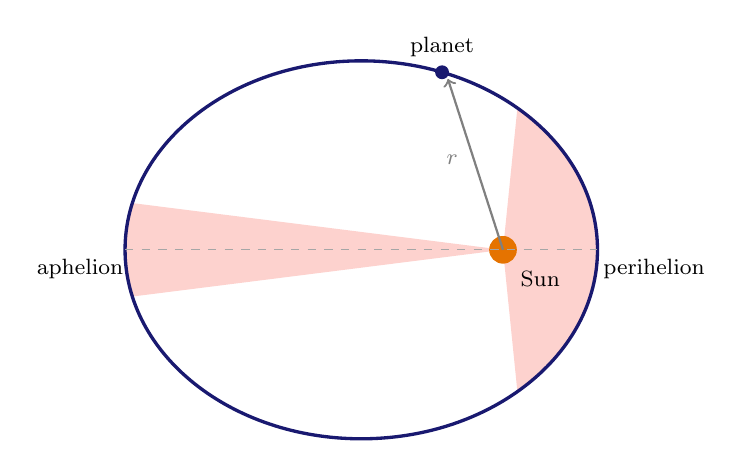
\begin{tikzpicture}[scale=1]
		% The two shaded sectors really do have equal area: sweeping the parametric
		% ellipse (3\cos t, 2.4\sin t) about the focus (1.8,0) gives
		% A = \tfrac12\int (7.2 - 4.32\cos t)\dd t, so the half-angles 48.63° at
		% perihelion and 14.32° at aphelion both enclose an area of 2.8688.
		\fill[Salmon!35]
		(1.8,0) -- plot[domain=-48.63:48.63, samples=60]
		({3*cos(\x)},{2.4*sin(\x)}) -- cycle;
		\fill[Salmon!35]
		(1.8,0) -- plot[domain=165.68:194.32, samples=40]
		({3*cos(\x)},{2.4*sin(\x)}) -- cycle;
		\draw[very thick, MidnightBlue] (0,0) ellipse (3 and 2.4);
		\fill[orange!90!black] (1.8,0) circle (5pt);
		\node[anchor=north west, font=\footnotesize] at (1.9,-0.15) {Sun};
		\fill[MidnightBlue] (1.026,2.255) circle (2.5pt);
		\draw[->, thick, gray] (1.8,0) -- (1.10,2.17);
		\node[gray, anchor=east, font=\footnotesize] at (1.35,1.15) {$\vb{r}$};
		\node[anchor=south, font=\footnotesize] at (1.026,2.33) {planet};
		\draw[dashed, gray!70] (-3,0) -- (3,0);
		\node[anchor=north east, font=\footnotesize] at (-2.9,0) {aphelion};
		\node[anchor=north west, font=\footnotesize] at (2.95,0) {perihelion};
	\end{tikzpicture}
	\caption{The two-body problem: an elliptical orbit with the Sun at a focus. The two
		shaded regions have equal area and are swept out in equal times --- so the planet
		moves fastest at perihelion.}
\end{figure}

\begin{moral}
	The two-body problem is \vocab{integrable}: it has enough conserved quantities
	(energy, the three components of angular momentum, and the Laplace--Runge--Lenz
	vector) to be solved completely in closed form. It is one of the very few nonlinear
	systems for which this is true.
\end{moral}

\subsubsection*{The three-body problem: the figure-eight orbit}

Add one more body and everything breaks.

\begin{fact}
	The three-body problem has no solution in closed form. Bruns (1887) and Poincaré
	(1890) showed that it admits no further algebraic conserved quantities of the kind
	that make the two-body problem solvable; Poincaré's work on it is the origin of the
	modern theory of chaos.
\end{fact}

What one can do instead is look for special solutions of high symmetry. Euler (1767)
found collinear ones and Lagrange (1772) found equilateral ones. In 1993 Cristopher Moore
found numerically, and in 2000 Alain Chenciner and Richard Montgomery proved rigorously,
that there is a solution in which three \emph{equal} masses chase one another around a
single figure-eight curve, each one-third of a period behind the last.

\begin{figure}[H]
	\centering
	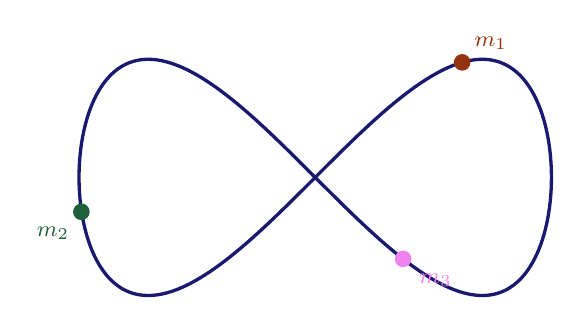
\begin{tikzpicture}[scale=1]
		\draw[very thick, MidnightBlue, domain=0:360, samples=200, smooth]
		plot ({3*cos(\x)},{1.5*sin(2*\x)});
		\fill[RawSienna] (1.866,1.461) circle (3pt);
		\fill[SeaGreen!70!black] (-2.970,-0.437) circle (3pt);
		\fill[Violet] (1.116,-1.035) circle (3pt);
		\node[RawSienna, anchor=south west, font=\footnotesize] at (1.9,1.5) {$m_1$};
		\node[SeaGreen!70!black, anchor=north east, font=\footnotesize]
		at (-3.0,-0.5) {$m_2$};
		\node[Violet, anchor=north west, font=\footnotesize] at (1.2,-1.1) {$m_3$};
	\end{tikzpicture}
	\caption{The figure-eight orbit of the three-body problem (schematic, drawn as a
		lemniscate): three equal masses travel the \emph{same} closed curve, spaced one
		third of a period apart. Discovered numerically by Moore (1993); existence proved
		by Chenciner and Montgomery (2000).}
\end{figure}

\subsection{The Lorenz System and Chaos}

\source{Lecture material; Boyce treats this in §9.8}

\begin{eg}[The Lorenz equations]
	In 1963 Edward Lorenz, a meteorologist at MIT, reduced a model of convection in the
	atmosphere to three ordinary differential equations:
	\begin{equation}\label{eq:lorenz}
		\begin{cases}
			\dot{x} = \sigma ( y - x ),   \\
			\dot{y} = x ( \rho - z ) - y, \\
			\dot{z} = x y - \beta z,
		\end{cases}
		\qquad
		\sigma = 10, \quad \beta = \frac{8}{3}, \quad \rho = 28.
	\end{equation}
\end{eg}

\begin{figure}[H]
	\centering
	\begin{tikzpicture}
		\begin{axis}[
				width=0.72\textwidth, height=6.4cm,
				xlabel={$x$}, ylabel={$z$},
				axis lines=left, xmin=-22, xmax=22, ymin=0, ymax=52,
			]
			\addplot[MidnightBlue, line width=0.15pt, opacity=0.8]
			table[x=x, y=z] {Figures/lorenz.dat};
		\end{axis}
	\end{tikzpicture}
	\caption{A single trajectory of the Lorenz system~\eqref{eq:lorenz}, projected onto
		the \(xz\)-plane: the ``butterfly'' strange attractor. The curve never closes and
		never repeats, yet stays forever in a bounded region.}
\end{figure}

\begin{observation}
	System~\eqref{eq:lorenz} is completely \emph{deterministic}: the state at time \(0\)
	determines the state at every later time. Nevertheless it is unpredictable in
	practice, because two initial conditions that differ by \(10^{-6}\) end up on opposite
	wings of the butterfly within a few dozen time units. Lorenz discovered this by
	accident, when he restarted a simulation from three-digit printed values instead of
	the six-digit values in the machine and got a completely different forecast. This
	\vocab{sensitive dependence on initial conditions} is the defining feature of
	\vocab{chaos}, popularly the \emph{butterfly effect}.
\end{observation}

\begin{remark}[Why three dimensions?]
	Chaos cannot happen sooner. For a scalar autonomous equation \(y' = f(y)\), solutions
	are monotone between equilibria, so they can only converge or blow up. In the plane,
	the Poincaré--Bendixson theorem says a bounded trajectory must approach an
	equilibrium or a closed orbit. Only from \emph{three} dimensions on is there enough
	room for a trajectory to wander forever without repeating itself.
\end{remark}

\begin{moral}
	``Solvable in closed form'' and ``understood'' are different things. Most of the
	equations that matter cannot be solved by the formulas of Chapter 2; the goal then
	shifts from finding \(y(t)\) to describing the \emph{qualitative} behaviour of the
	solutions --- equilibria, stability, periodicity, attractors.
\end{moral}

\section{Classification of Differential Equations}

\source{Boyce §1.3}

Mastering the following vocabulary is essential for selecting appropriate solution
methods.

\subsection{Ordinary and Partial Differential Equations}

\begin{definition}[ODE, PDE]
	If the unknown function depends on a \emph{single} independent variable, only ordinary
	derivatives appear and the equation is an \vocab{ordinary differential equation}
	(ODE). If it depends on \emph{several} independent variables, the derivatives are
	partial derivatives and the equation is a \vocab{partial differential equation} (PDE).
\end{definition}

\begin{eg}
	All equations so far have been ODEs. Another is the equation
	\[
		L\frac{\dd^2 Q(t)}{\dd t^2} + R \frac{\dd Q(t)}{\dd t} + \frac{1}{C} Q(t) = E(t)
	\]
	for the charge \(Q(t)\) on a capacitor in a circuit with capacitance \(C\),
	resistance \(R\) and inductance \(L\). Typical PDEs are the \vocab{heat conduction
		equation}
	\[
		\alpha^2 \pdv[2]{u(x,t)}{x} = \pdv{u(x,t)}{t}
	\]
	and the \vocab{wave equation}
	\[
		a^2 \pdv[2]{u(x,t)}{x} = \pdv[2]{u(x,t)}{t},
	\]
	in which \(u\) depends on the two independent variables \(x\) and \(t\), and
	\(\alpha^2, a^2\) are physical constants.
\end{eg}

\subsection{Order}

\begin{definition}[Order]
	The \vocab{order} of a differential equation is the order of the highest derivative
	appearing in it. The general \(n\)th order ODE is
	\begin{equation}\label{eq:implicit-nth}
		F\left( t, u(t), u'(t), \dots, u^{(n)}(t) \right) = 0.
	\end{equation}
\end{definition}

\begin{notation}
	It is customary to write \(y\) for \(u(t)\), and \(y', y'', \dots, y^{(n)}\) for
	\(u'(t), u''(t), \dots, u^{(n)}(t)\), so that~\eqref{eq:implicit-nth} becomes
	\[
		F\left( t, y, y', \dots, y^{(n)} \right) = 0.
	\]
\end{notation}

\begin{eg}
	\(y''' + 2e^{t} y'' + y y' = t^4\) is a third-order equation. The
	equations~\eqref{eq:twobody} of celestial mechanics are second order.
\end{eg}

We will always assume that~\eqref{eq:implicit-nth} can be solved for the highest
derivative, giving the \vocab{explicit} (or \vocab{normal}) form
\begin{equation}\label{eq:explicit-nth}
	y^{(n)} = f\left( t, y, y', \dots, y^{(n-1)} \right).
\end{equation}

\begin{remark}[Where the ambiguity comes from]
	Passing from the implicit equation~\eqref{eq:implicit-nth} to the explicit
	form~\eqref{eq:explicit-nth} is not just rearranging terms: it means \emph{solving}
	the equation
	\[
		F\left( t, y, \dots, y^{(n-1)}, y^{(n)} \right) = 0
	\]
	for the last variable \(y^{(n)}\), treating everything else as known. That is an
	algebraic step, and an algebraic equation can have more than one root. So a single
	implicit
	equation of the form~\eqref{eq:implicit-nth} need not determine a single explicit
	equation of the form~\eqref{eq:explicit-nth} --- it may split into several, one per
	root.
\end{remark}

\begin{eg}
	The equation \((y')^2 + t y' + 4y = 0\) is quadratic in the unknown \(y'\). Applying
	the quadratic formula (with \(t\) and \(y\) playing the role of the coefficients),
	\[
		y' = \frac{-t \pm \sqrt{t^2 - 16y}}{2},
	\]
	which is really \emph{two} different explicit equations,
	\[
		y' = \frac{-t + \sqrt{t^2 - 16y}}{2}
		\qquad\text{and}\qquad
		y' = \frac{-t - \sqrt{t^2 - 16y}}{2},
	\]
	each defined only where \(t^2 \geq 16y\) (so the square root is real), and each with
	a \emph{different} function \(f(t,y)\) on the right-hand side. Either one, substituted
	back in, satisfies the original implicit equation --- but the two are genuinely
	different differential equations, and in general have different solutions \(y(t)\).
\end{eg}

\begin{remark}
	This is what ``assume~\eqref{eq:implicit-nth} can be solved for the highest
	derivative'' really commits us to: pick \emph{one} of the roots (here, one of the two
	square-root branches, on the region \(t^2 \geq 16y\) where it is defined) and take
	that fixed choice as \(f\) in~\eqref{eq:explicit-nth}. Everything afterwards --- in
	particular the definition of \emph{solution} below --- refers to that one explicit
	equation, not to the implicit equation we started from.
\end{remark}

\subsection{Scalar Equations and Systems of Equations}

\begin{definition}[System]
	If a single unknown function is to be determined, one equation suffices and we speak
	of a \vocab{scalar equation}. If two or more unknown functions are involved, a
	\vocab{system} of differential equations is required.
\end{definition}

\begin{eg}[Lotka--Volterra / predator--prey equations]
	\[
		\begin{cases}
			\dfrac{\dd x}{\dd t} = ax - \alpha xy, \\[1.2ex]
			\dfrac{\dd y}{\dd t} = -cy + \gamma xy,
		\end{cases}
	\]
	where \(x(t)\) and \(y(t)\) are the populations of prey and predator respectively and
	\(a, \alpha, c, \gamma > 0\) are empirical constants. The Lorenz
	system~\eqref{eq:lorenz} is a system of three equations; the two-body
	problem~\eqref{eq:twobody} a system of six.
\end{eg}

\begin{remark}
	The two classifications interact: any scalar equation of order \(n\) can be rewritten
	as a \emph{first-order system} of \(n\) equations, by taking
	\(y_1 = y,\ y_2 = y',\ \dots,\ y_n = y^{(n-1)}\). This is why the theory of
	first-order systems is the central object of the subject.
\end{remark}

\subsection{Linear and Nonlinear Equations}

\begin{definition}[Linear equation]
	The ODE \(F(t, y, y', \dots, y^{(n)}) = 0\) is \vocab{linear} if \(F\) is a linear
	function of the variables \(y, y', \dots, y^{(n)}\). Thus the general linear ODE of
	order \(n\) is
	\begin{equation}\label{eq:linear-n}
		a_0(t) y^{(n)} + a_1(t) y^{(n-1)} + \dots + a_n(t) y = g(t).
	\end{equation}
	An equation not of the form~\eqref{eq:linear-n} is \vocab{nonlinear}.
\end{definition}

\begin{remark}
	Note that no condition is imposed on how \(t\) enters: the coefficients \(a_i(t)\) and
	the right-hand side \(g(t)\) may be arbitrary functions of \(t\). Linearity concerns
	only \(y\) and its derivatives.
\end{remark}

\begin{eg}
	\(y''' + 2e^t y'' + yy' = t^4\) is nonlinear, because of the term \(yy'\). Each
	Lotka--Volterra equation is nonlinear because of the products \(xy\), and each Lorenz
	equation because of \(xz\) and \(xy\).
\end{eg}

\begin{eg}[The oscillating pendulum]
	The angle \(\theta = \theta(t)\) that a pendulum of length \(L\) makes with the
	vertical satisfies
	\begin{equation}\label{eq:pendulum}
		\frac{\dd^2 \theta}{\dd t^2} + \frac{g}{L} \sin\theta = 0,
	\end{equation}
	which is nonlinear because of the term \(\sin\theta\).
\end{eg}

\begin{definition}[Linearization]
	Approximating a nonlinear equation by a linear one is called \vocab{linearization}.
\end{definition}

\begin{eg}
	For small \(\theta\) we have \(\sin\theta \approx \theta\), so~\eqref{eq:pendulum}
	is approximated by the linear equation
	\[
		\frac{\dd^2\theta}{\dd t^2} + \frac{g}{L}\theta = 0.
	\]
\end{eg}

\begin{moral}
	The theory and methods for linear equations are highly developed; for nonlinear
	equations the theory is more complicated and the methods less satisfactory.
	Fortunately, many significant problems are linear or can be usefully linearized ---
	but, as the Lorenz system shows, many phenomena genuinely require nonlinear equations.
\end{moral}

\subsection{Solutions}

\begin{definition}[Solution]\label{def:solution}
	A \vocab{solution} of the \(n\)th order ODE~\eqref{eq:explicit-nth} on an interval
	\(\alpha < t < \beta\) is a function \(\varphi\) such that
	\(\varphi', \varphi'', \dots, \varphi^{(n)}\) exist and satisfy
	\[
		\varphi^{(n)}(t) = f\left( t, \varphi(t), \varphi'(t), \dots,
		\varphi^{(n-1)}(t) \right)
	\]
	for every \(t\) with \(\alpha < t < \beta\).
\end{definition}

Unless stated otherwise we take \(f\) real-valued and seek real-valued solutions.

\begin{observation}
	Finding a solution can be very hard, but \emph{checking} a candidate is usually easy:
	just substitute it into the equation. For instance, \(y_1(t) = \cos t\) satisfies
	\(y'' + y = 0\) for all \(t\), since \(y_1'(t) = -\sin t\) and \(y_1''(t) = -\cos t\);
	likewise \(y_2(t) = \sin t\) is a solution. Verifying a proposed solution is a habit
	worth acquiring.
\end{observation}

\subsection{Three Fundamental Questions}

\begin{question}[Existence]
	Does an equation of the form~\eqref{eq:explicit-nth} always have a solution?
\end{question}

The answer is \textbf{no}: merely writing down such an equation does not guarantee a
function satisfying it. Existence theorems state that under suitable restrictions on
\(f\), solutions do exist. This is not a purely theoretical concern: we would rather know
in advance than waste effort on an unsolvable problem, and if a sensible physical problem
yields an equation with no solution, something is wrong with the formulation.

\begin{question}[Uniqueness]
	If solutions exist, how many are there, and what extra conditions single one out?
\end{question}

Solutions generally contain arbitrary constants of integration, so there is typically an
infinite family. Prescribing \(y\) at a point determines the constant --- but this does
not by itself rule out \emph{other} solutions with the same prescribed value. If we know
the problem has a unique solution and we have found one, we are finished; otherwise we
should keep searching.

\begin{question}[Determination of solutions]
	Given~\eqref{eq:explicit-nth}, can we actually determine a solution, and if so, how?
\end{question}

Finding a solution simultaneously answers the existence question. But without existence
theory one might, for example, use a computer to produce a numerical approximation to a
``solution'' that does not exist. Moreover, even when a solution exists it may not be
expressible in terms of elementary functions --- polynomial, trigonometric, exponential,
logarithmic and hyperbolic --- and unfortunately this is the situation for \emph{most}
differential equations. Hence we study both exact elementary methods for simple problems
and approximation methods of a more general nature.

\begin{moral}
	Always try to combine numerical, graphical and analytical methods, so as to attain
	maximum understanding of the behaviour of the solution and of the process it models.
\end{moral}

\chapter{First-Order Differential Equations}

This chapter deals with equations of first order
\[
	\frac{\dd y}{\dd t} = f(t,y),
\]
where \(f\) is a given function of two variables. For an arbitrary \(f\) there is
\emph{no} general method of solution in terms of elementary functions; instead we
describe several methods, each applicable to a certain subclass. The most important are
\textbf{linear} equations (\autoref{sec:linear}), \textbf{separable} equations
(\autoref{sec:separable}), and \textbf{exact} equations (Boyce §2.6).

\section{Linear Differential Equations; Method of Integrating Factors}\label{sec:linear}

\source{Boyce §2.1}

\begin{definition}[First-order linear equation]
	If \(f\) depends linearly on \(y\), then \(\dd y/\dd t = f(t,y)\) is a
	\vocab{first-order linear differential equation}. We write it in the \vocab{standard
		form}
	\begin{equation}\label{eq:std}
		\frac{\dd y}{\dd t} + p(t) y = g(t),
	\end{equation}
	where \(p\) and \(g\) are given functions of \(t\).
\end{definition}

\begin{remark}
	Sometimes it is convenient to write the equation as
	\(P(t) y' + Q(t) y = G(t)\); as long as \(P(t) \neq 0\), dividing by \(P(t)\) returns
	it to the standard form~\eqref{eq:std}. \textbf{Always convert to standard form before
		reading off \(p\) and \(g\).}
\end{remark}

\begin{remark}
	\autoref{thm:linear-const} solved the special case \(p, g\) constant. We now allow
	both to depend on \(t\), which no longer yields to the trick used there.
\end{remark}

Occasionally the equation can be integrated at once.

\begin{eg}
	Solve \((4 + t^2) \dfrac{\dd y}{\dd t} + 2ty = 4t\).
\end{eg}

\begin{proof}[Solution]
	The left-hand side is exactly the derivative of a product:
	\[
		(4 + t^2)\frac{\dd y}{\dd t} + 2ty = \frac{\dd}{\dd t}\left[ (4 + t^2) y \right].
	\]
	So the equation reads \(\dfrac{\dd}{\dd t}\left[ (4+t^2) y \right] = 4t\), and even
	though \(y\) is unknown we may integrate both sides:
	\[
		(4 + t^2) y = 2t^2 + c
		\implies
		y = \frac{2t^2}{4 + t^2} + \frac{c}{4 + t^2}.
	\]
\end{proof}

Most equations are not so lucky: the left-hand side is usually not the derivative of a
product. Leibniz's idea was to \emph{make} it one.

\begin{definition}[Integrating factor]
	A function \(\mu(t)\) such that multiplying~\eqref{eq:std} by \(\mu(t)\) turns the
	left-hand side into \(\dfrac{\dd}{\dd t}\left[ \mu(t) y \right]\) is called an
	\vocab{integrating factor} for~\eqref{eq:std}.
\end{definition}

\begin{eg}
	Find the general solution of
	\(\dfrac{\dd y}{\dd t} + \dfrac{1}{2} y = \dfrac{1}{2} e^{t/3}\), and the particular
	solution through \((0,1)\).
\end{eg}

\begin{proof}[Solution]
	Multiply by an as-yet-undetermined \(\mu(t)\):
	\begin{equation}\label{eq:mu-eg}
		\mu(t) \frac{\dd y}{\dd t} + \frac{1}{2}\mu(t) y
		= \frac{1}{2}\mu(t) e^{t/3}.
	\end{equation}
	For any differentiable function \(\mu\),
	\[
		\frac{\dd}{\dd t}\left( \mu(t) y \right)
		= \mu(t) \frac{\dd y}{\dd t} + \frac{\dd \mu(t)}{\dd t} y,
	\]
	so the left-hand side of~\eqref{eq:mu-eg} is such a derivative precisely when
	\[
		\frac{\dd \mu(t)}{\dd t} = \frac{1}{2} \mu(t)
		\iff \frac{1}{\mu(t)} \frac{\dd \mu(t)}{\dd t} = \frac{1}{2}
		\iff \frac{\dd}{\dd t} \ln\abs{\mu(t)} = \frac{1}{2},
	\]
	whence \(\mu(t) = c_0 e^{t/2}\) for an arbitrary constant \(c_0\). We do not need the
	most general integrating factor, so take \(c_0 = 1\) and \(\mu(t) = e^{t/2}\). Then
	\[
		\frac{\dd}{\dd t}\left( e^{t/2} y \right) = \frac{1}{2} e^{5t/6}
		\implies e^{t/2} y = \frac{3}{5} e^{5t/6} + c,
	\]
	and therefore the general solution is
	\[
		y = \frac{3}{5} e^{t/3} + c e^{-t/2}.
	\]
	Setting \(t = 0\), \(y = 1\) gives \(1 = 3/5 + c\), so \(c = 2/5\) and the desired
	solution is \(y = \frac{3}{5} e^{t/3} + \frac{2}{5} e^{-t/2}\).
\end{proof}

\begin{figure}[H]
	\centering
	\begin{tikzpicture}
		\begin{axis}[
				width=0.66\textwidth, height=6cm,
				xlabel={$t$}, ylabel={$y$},
				xmin=0, xmax=6, ymin=-2, ymax=4,
				axis lines=middle,
				every axis x label/.style={at={(ticklabel* cs:1.0)},anchor=west},
				every axis y label/.style={at={(ticklabel* cs:1.0)},anchor=south},
			]
			\foreach \X in {0.25,0.75,...,5.75}{
					\foreach \Y in {-2,-1.5,...,4}{
							\pgfmathsetmacro{\Sl}{0.5*exp(\X/3)-0.5*\Y}%
							\slopemark{gray!70}{\X}{\Y}{\Sl}{1.76}{1.0}
						}
				}
			\foreach \c in {-2,-1,1,2}{
					\addplot[thick, MidnightBlue!70, domain=0:6, samples=100]
					{0.6*exp(x/3) + \c*exp(-x/2)};
				}
			\addplot[very thick, correct, domain=0:6, samples=100]
			{0.6*exp(x/3) + 0.4*exp(-x/2)};
		\end{axis}
	\end{tikzpicture}
	\caption{Direction field and integral curves of
		\(y' + \frac12 y = \frac12 e^{t/3}\); the green curve is the solution through
		\((0,1)\).}
\end{figure}

\subsection{The Constant-Coefficient Case}

For \(\dfrac{\dd y}{\dd t} + ay = g(t)\) with \(a\) constant, the integrating factor must
satisfy \(\dd\mu/\dd t = a\mu\), so \(\mu(t) = e^{at}\). Then
\[
	\frac{\dd}{\dd t}\left( e^{at} y \right) = e^{at} g(t)
	\implies e^{at} y = \int e^{at} g(t) \dd t + c.
\]
For complicated \(g\) the integral may have to be left unevaluated, in which case
\begin{equation}\label{eq:const-coeff-sol}
	y = e^{-at} \int_{t_0}^{t} e^{as} g(s) \dd s + c e^{-at}.
\end{equation}

\begin{note}
	In~\eqref{eq:const-coeff-sol} we use \(s\) for the integration variable to distinguish
	it from the independent variable \(t\), and \(t_0\) is any convenient lower limit. The
	choice of \(t_0\) changes the value of \(c\) --- indeed \(c = y(t_0) e^{a t_0}\) ---
	but not the solution itself.
\end{note}

\begin{eg}
	Find the general solution of \(\dfrac{\dd y}{\dd t} - 2y = 4 - t\) and discuss the
	behaviour as \(t \to \infty\).
\end{eg}

\begin{proof}[Solution]
	Here \(a = -2\), so \(\mu(t) = e^{-2t}\) and
	\[
		\frac{\dd}{\dd t}\left( e^{-2t} y \right) = 4e^{-2t} - te^{-2t}.
	\]
	Integrating (by parts on the last term),
	\[
		e^{-2t} y = -2e^{-2t} + \frac{1}{2}te^{-2t} + \frac{1}{4}e^{-2t} + c,
	\]
	so the general solution is
	\[
		y = -\frac{7}{4} + \frac{1}{2}t + c e^{2t}.
	\]
	The behaviour for large \(t\) is dominated by \(ce^{2t}\). If \(c \neq 0\) the
	solution grows exponentially with the sign of \(c\); all such solutions diverge. The
	borderline case is \(c = 0\), i.e.\ \(y(0) = -7/4\), for which
	\(y = -\frac74 + \frac12 t\) grows only \emph{linearly}.
\end{proof}

\subsection{The General Case}

\begin{theorem}[Method of integrating factors]\label{thm:integrating-factor}
	Consider the first-order linear equation in standard form
	\[
		\frac{\dd y}{\dd t} + p(t) y = g(t).
	\]
	Then
	\begin{equation}\label{eq:mu}
		\mu(t) = \exp\left( \int p(t) \dd t \right)
	\end{equation}
	is an integrating factor, and the general solution is
	\begin{equation}\label{eq:gen-lin-sol}
		y = \frac{1}{\mu(t)}\left[ \int_{t_0}^{t} \mu(s) g(s) \dd s + c \right].
	\end{equation}
\end{theorem}

\begin{proof}
	Multiplying the equation by \(\mu(t)\) gives
	\begin{equation}\label{eq:mu-general}
		\mu(t) \frac{\dd y}{\dd t} + p(t) \mu(t) y = \mu(t) g(t),
	\end{equation}
	whose left-hand side is \(\dfrac{\dd}{\dd t}(\mu(t) y)\) precisely when
	\[
		\frac{\dd \mu(t)}{\dd t} = p(t)\mu(t).
	\]
	Assuming temporarily that \(\mu(t) > 0\), this says
	\(\dfrac{1}{\mu(t)}\dfrac{\dd\mu(t)}{\dd t} = p(t)\), so
	\(\ln\abs{\mu(t)} = \int p(t) \dd t + k\). Choosing \(k = 0\) gives the simplest
	choice~\eqref{eq:mu}, which is indeed positive for all \(t\), as assumed. Then
	equation~\eqref{eq:mu-general} reads
	\(\dfrac{\dd}{\dd t}(\mu(t) y) = \mu(t) g(t)\), and integrating gives
	\(\mu(t) y = \int \mu(t) g(t) \dd t + c\), which is~\eqref{eq:gen-lin-sol}.
\end{proof}

\begin{remark}
	Observe that~\eqref{eq:gen-lin-sol} involves \textbf{two} integrations: one to obtain
	\(\mu(t)\) from~\eqref{eq:mu}, and another to obtain \(y\).
\end{remark}

\begin{eg}
	Solve the initial value problem \(ty' + 2y = 4t^2\), \(y(1) = 2\).
\end{eg}

\begin{proof}[Solution]
	First convert to standard form (dividing by \(t\)):
	\[
		y' + \frac{2}{t} y = 4t,
	\]
	so \(p(t) = 2/t\) and \(g(t) = 4t\). The integrating factor is
	\[
		\mu(t) = \exp\left( \int \frac{2}{t} \dd t \right) = e^{2\ln\abs{t}} = t^2.
	\]
	Multiplying through, \(t^2 y' + 2ty = (t^2 y)' = 4t^3\), so
	\(t^2 y = \int 4t^3 \dd t = t^4 + c\), and for \(t > 0\),
	\[
		y = t^2 + \frac{c}{t^2}.
	\]
	The initial condition gives \(2 = 1 + c\), so \(c = 1\) and
	\[
		y = t^2 + \frac{1}{t^2}, \qquad t > 0.
	\]
\end{proof}

\begin{remark}[Interval of validity]\label{rmk:interval-validity}
	This is the first example in which the solution fails to exist for all \(t\): the
	solution becomes unbounded as \(t \to 0^{+}\), so it is restricted to
	\(0 < t < \infty\). It is worth being precise about \emph{why} \(t < 0\) is excluded,
	since it is \textbf{not} for the same reason as \autoref{rmk:logcare} --- that one is
	about an algebraic equation for \(y'\) having several roots; nothing like that is
	happening here.

	First, check directly that \(t < 0\) is not an algebra problem: substituting
	\(y = t^2 + 1/t^2\) into the \emph{original} equation \(ty' + 2y = 4t^2\) gives
	\[
		t\!\left( 2t - \frac{2}{t^3} \right) + 2\left( t^2 + \frac{1}{t^2} \right)
		= 2t^2 - \frac{2}{t^2} + 2t^2 + \frac{2}{t^2} = 4t^2,
	\]
	which holds for \emph{every} \(t \neq 0\), negative \(t\) included --- there is no
	hidden sign restriction, no square root, nothing multivalued. So the formula itself
	is perfectly happy on \(t < 0\).

	The real obstruction is \emph{connectedness}. Dividing by \(t\) to reach standard
	form is only legal for \(t \neq 0\), and \(p(t) = 2/t\) genuinely blows up there; so
	the domain on which our equation makes sense at all, \(t \neq 0\), is not one
	interval but \emph{two}: \((-\infty, 0)\) and \((0, \infty)\), with no way to pass
	between them. Every integral curve \(y = t^2 + c/t^2\) with \(c \neq 0\) shares this
	feature --- it blows up as \(t \to 0\) from whichever side it lives on --- so no
	solution curve can be continued across \(t = 0\) to link the two sides into a single
	differentiable function. But \autoref{def:solution} \emph{requires} a solution to be
	one function on one interval \(\alpha < t < \beta\). Since the initial point
	\(t_0 = 1\) lies in \((0,\infty)\), that is the only interval available to the
	solution of \emph{this} IVP, and \(t < 0\) is simply outside its domain --- not
	because the formula fails there, but because that region belongs to a different,
	disconnected piece of the picture.

	This also means the constant on the two sides need not match. Because
	\(y = t^2 + c/t^2\) is an \emph{even} function of \(t\) for every fixed \(c\), the
	left half of the plot below happens to look like a mirror image of the right half ---
	but that symmetry is an accident of this particular formula, not a consequence of the
	initial condition. Nothing forces the branch on \(t < 0\) to use \(c = 1\); any other
	constant would glue on there just as validly, since the initial condition
	\(y(1) = 2\) says nothing at all about behaviour on \(t < 0\).
\end{remark}

\begin{figure}[H]
	\centering
	\begin{tikzpicture}
		\begin{axis}[
				width=0.68\textwidth, height=6.2cm,
				xlabel={$t$}, ylabel={$y$},
				xmin=-2.3, xmax=2.3, ymin=-1.5, ymax=6.3,
				axis lines=middle,
				every axis x label/.style={at={(ticklabel* cs:1.0)},anchor=west},
				every axis y label/.style={at={(ticklabel* cs:1.0)},anchor=south},
			]
			\draw[gray, dashed] (axis cs:0,-1.5) -- (axis cs:0,6.3);
			\foreach \C in {-1,0,2}{
					\addplot[gray!55, thin, restrict y to domain=-2:6.3,
						domain=0.32:2.3, samples=80] {x^2 + \C/x^2};
					\addplot[gray!55, thin, restrict y to domain=-2:6.3,
						domain=-2.3:-0.32, samples=80] {x^2 + \C/x^2};
				}
			\addplot[very thick, correct, restrict y to domain=-2:6.3,
				domain=0.32:2.3, samples=100] {x^2 + 1/x^2};
			\addplot[only marks, mark=*, mark size=1.6pt, correct]
			coordinates {(1,2)};
			\addplot[very thick, orange!85!black, restrict y to domain=-2:6.3,
				domain=-2.3:-0.32, samples=100] {x^2 + 3/x^2};
			\node[gray, anchor=south, font=\footnotesize] at (axis cs:0,6.0) {$t=0$};
		\end{axis}
	\end{tikzpicture}
	\caption{No integral curve of \(ty' + 2y = 4t^2\) crosses \(t = 0\) (dashed): every
		curve with \(c \neq 0\) blows up there. The green curve, \(c = 1\), is the solution
		of the IVP \(y(1) = 2\); it lives only on \(t > 0\). The formula happens to be even
		in \(t\), so the same shapes reappear for \(t < 0\) (thin gray) --- but the initial
		condition never touches that side, so the orange curve (\(c = 3\)) would glue on
		just as legitimately as any other choice.}
\end{figure}

\begin{observation}[The one exception]
	With \(y(1) = y_0\) instead of \(y(1)=2\), the same computation gives
	\(c = y_0 - 1\), so \(y = t^2 + (y_0-1)/t^2\). Every value of \(c\) makes the curve
	blow up at \(t=0\) --- \emph{except} \(c = 0\), i.e.\ \(y_0 = 1\), for which the
	singular term vanishes and \(y = t^2\) is perfectly smooth at \(t = 0\) (indeed
	\(y=t^2\) solves \(ty'+2y=4t^2\) for \emph{all} \(t \in \mathbb{R}\), no restriction
	needed). This is the one curve in the whole family that manages to cross from
	\(t>0\) to \(t<0\) without a jump. Solutions with \(c > 0\) shoot up to \(+\infty\)
	as \(t \to 0^{+}\) (asymptotic to the positive \(y\)-axis) and those with \(c<0\) to
	\(-\infty\) (the negative \(y\)-axis) --- exactly what the thin gray curves in the
	figure show.
\end{observation}

\begin{eg}
	Solve the initial value problem \(2y' + ty = 2\), \(y(0) = 1\).
\end{eg}

\begin{proof}[Solution]
	In standard form, \(y' + \frac{t}{2}y = 1\), so \(p(t) = t/2\) and
	\(\mu(t) = \exp(t^2/4)\). Then
	\[
		\frac{\dd}{\dd t}\left( e^{t^2/4} y \right) = e^{t^2/4}
		\implies e^{t^2/4} y = \int e^{t^2/4} \dd t + c.
	\]
	The integral \(\int e^{t^2/4}\dd t\) \textbf{cannot} be evaluated in terms of
	elementary functions, so we leave it. Choosing the initial point \(t = 0\) as the
	lower limit,
	\[
		y = e^{-t^2/4}\int_{0}^{t} e^{s^2/4}\dd s + c e^{-t^2/4}.
	\]
	Setting \(t = 0\), \(y = 1\) gives \(1 = 0 + c\), so \(c = 1\).
\end{proof}

\begin{moral}
	Sometimes the solution must be left in terms of an integral. This is at most a slight
	inconvenience rather than a serious obstacle: for each \(t\) the integral is a
	\emph{definite} integral, which can be approximated numerically to any desired
	accuracy.
\end{moral}
